\documentclass[a4paper,12pt]{article}
%\usepackage[utf8x]{inputenc}
\usepackage{graphicx}

%opening
\title{SDES}
\author{MEGH}

\begin{document}

% \maketitle

% \begin{abstract}
% hi
% 
% 
% \end{abstract}

\section{Simulator Design Overview}

Figure \ref{class_struct}  shows the overall class structure of the simulator design. Class \emph{LG} \emph{i.e.} Logic Gate is the abstract class for implementation of the all other basic gates. Instance of class \emph{LG} cannot be created. class \emph{GATE1} and \emph{GATE2} are derived from class \emph{LG}. Class \emph{GATE1} stands for the one input one output gates and class \emph{GATE2} stands for two input and two out gates. Class \emph{Connector} is used for connecting different basic components to create combinational and sequential circuits. Details of all classes are described in further sections.


  \begin{figure}[!h]
   \begin{center}
   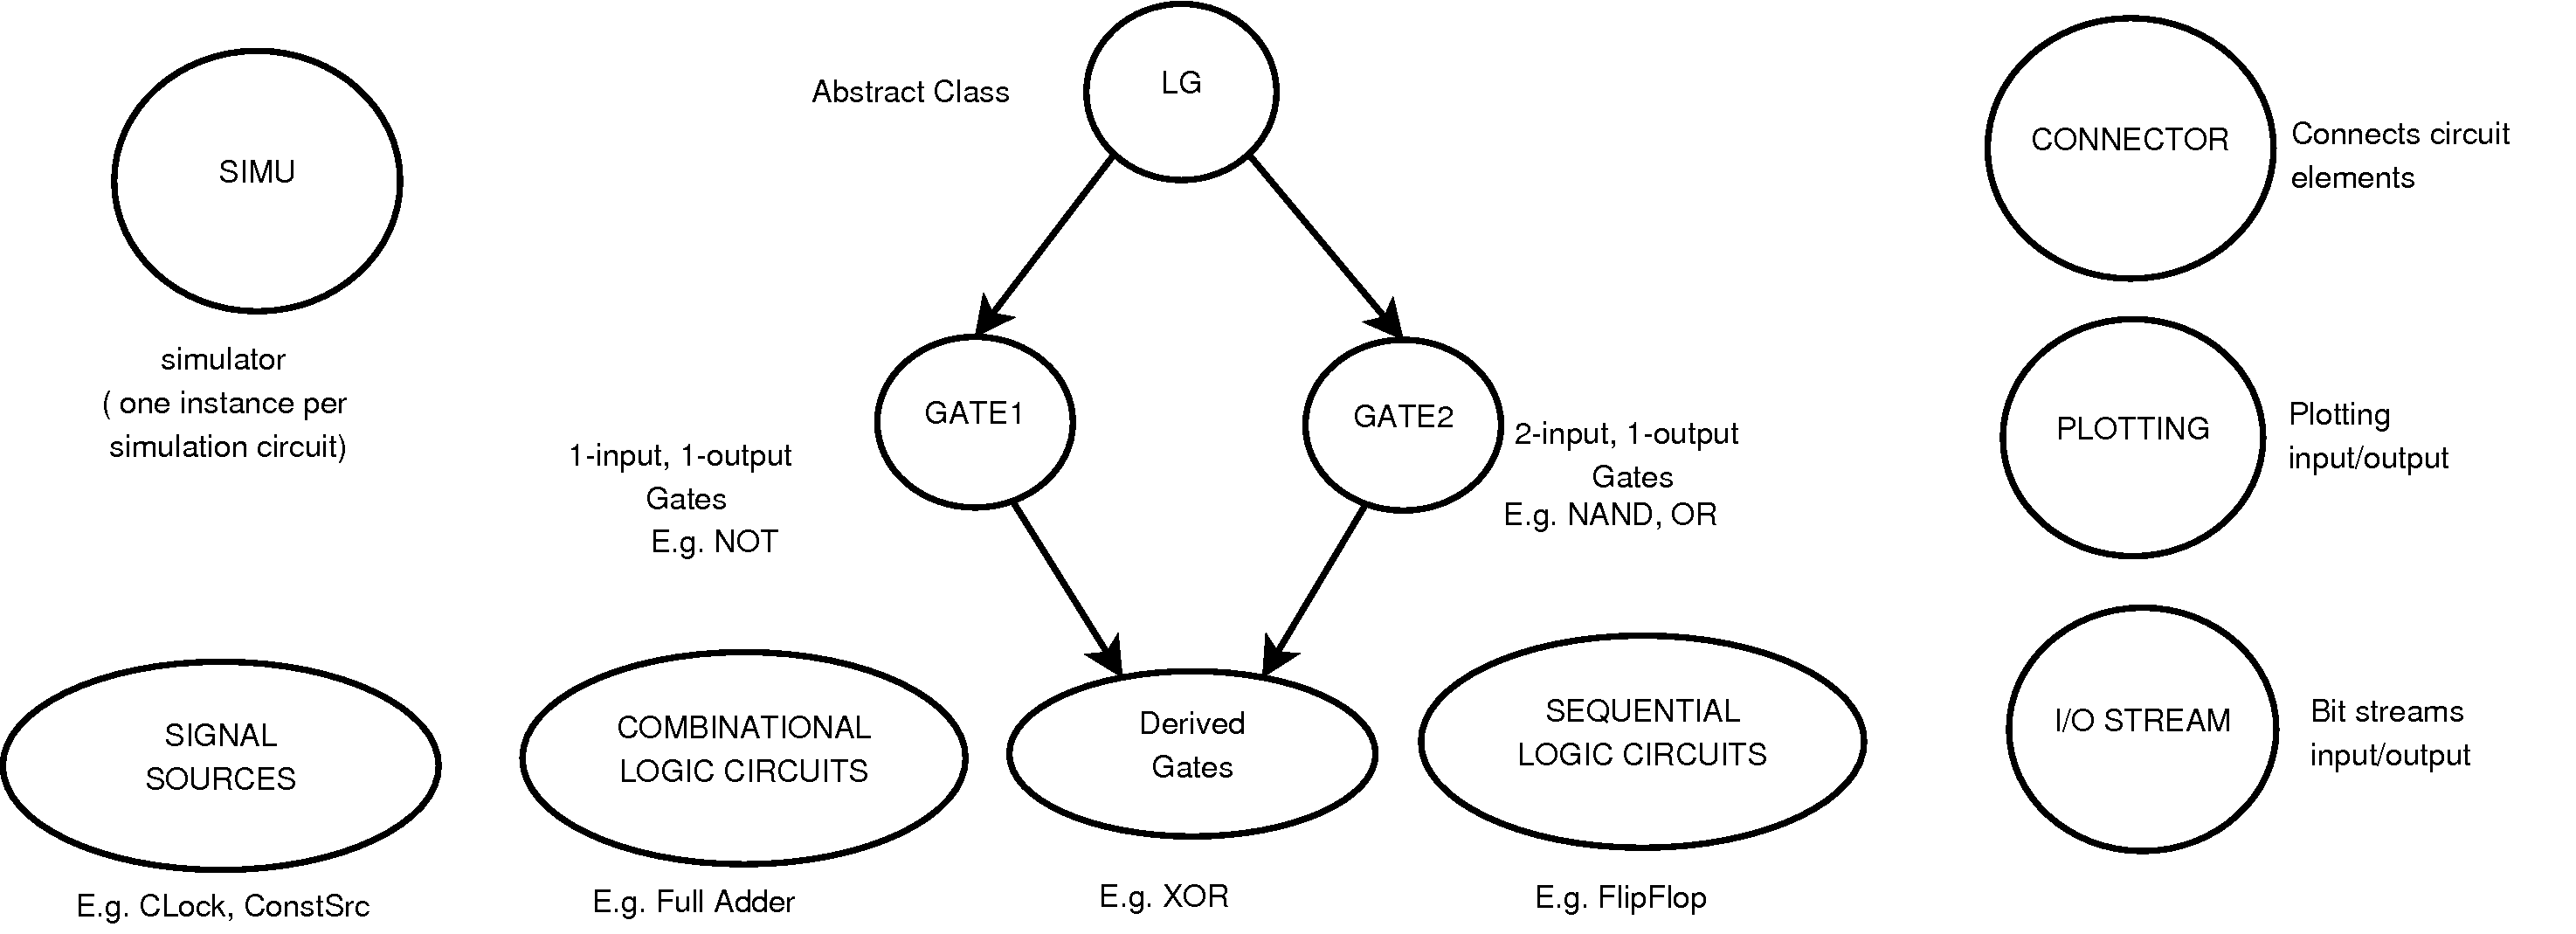
\includegraphics[scale=0.3]{class3.png}
    \caption{{Class Structure}}
  \label{class_struct}
  \end{center}
  \end{figure}

Class \emph{SIMU} is the central class of the \emph{pydlcs} simulator. It monitors the whole circuit operations and provides clock to different elements of the circuit. Its main functions are,
\begin{itemize}
 \item Provide system clock to circuit elements
 \item Plotting input and output graphs
 \item Save the results and plots
 \item Monitor and control i/o streams
 \item Circuit debug option
\end{itemize}

Figure \ref{simu_class} shows the \emph{SIMU} class details. We are going to describe the usage of this class's object in upcoming sections.\\



\begin{figure}[!h]
   \begin{center}
   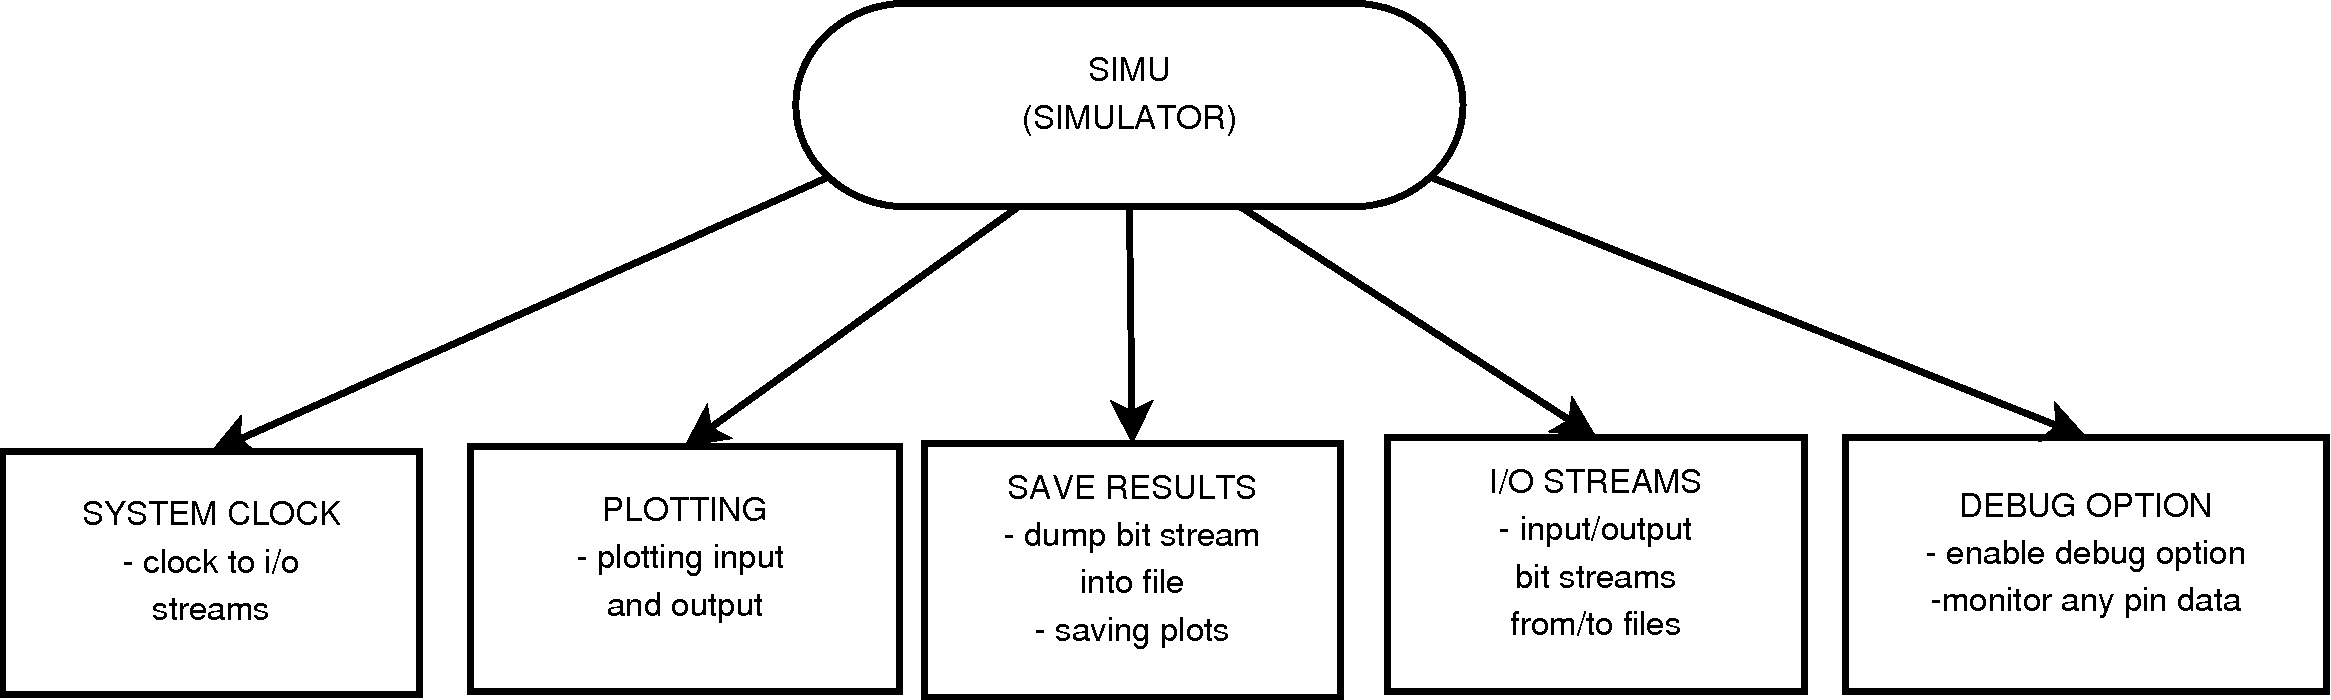
\includegraphics[scale=0.35]{simu_model.png}
    \caption{{Simulator Class Details}}
  \label{simu_class}
  \end{center}
  \end{figure}


Figure \ref{syst_model} shows the system model of the \emph{pydlcs} simulator. Simulator takes the bit-streams as an input form files specified. \emph{Istream} is the class defined for the providing the input facility from files. Each \emph{Istream} object is connected to one file on one side and can supply bit-stream to any number of gates of the circuit on other side. \emph{Ostream} is class defined for providing facility of writing result of simulation into the file specified. \emph{Ostream} class object is connected to circuit pin from one side and pins data is logged into the file specified on other side. Both classes, \emph{Istream} and \emph{Ostream}, need to provide system clock for their operation. Figure \ref{iostream} shows the \emph{i/ostream} operational model. Their are different flags in \emph{SIMU} class that we need to set for enabling different options \emph{e.g.} for enabling annotation  of plots we need to set flag \emph{pannotate} in \emph{SIMU} object. Flags details are as bellow,
\begin{itemize}
 \item \emph{plots} - Enable plots
 \item \emph{pannotate} - Enable plot annotation
 \item \emph{pclk} - Enable plotting system clock
 \item \emph{start} - Start the simulation flag
 \item \emph{stop} - Stop simulation flag
 \item \emph{debug} - Enable debugging
 \item \emph{step} - Enable step execution
\end{itemize}

 There should be only one instance of \emph{SIMU} class per circuit description file. Introduction to writing circuit description file is given in upcoming sections. 

\begin{figure}[!h]
   \begin{center}
   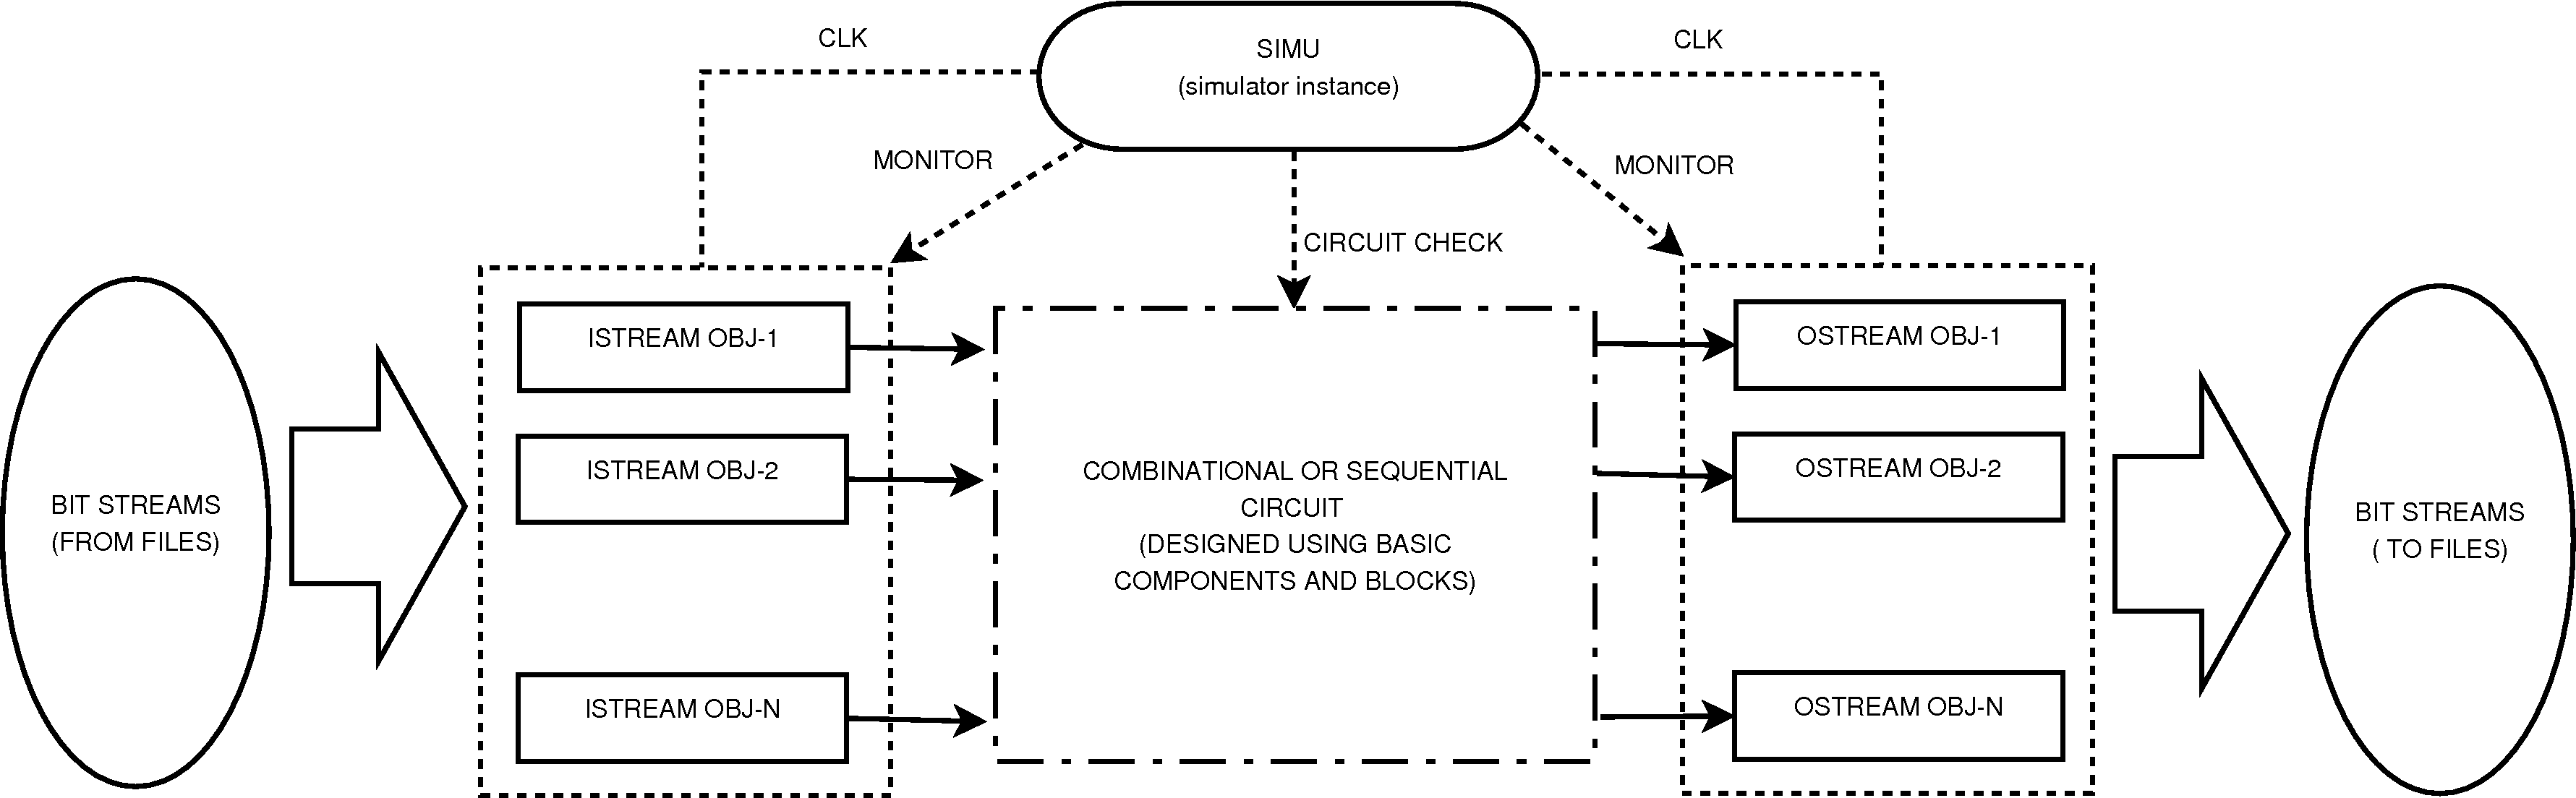
\includegraphics[scale=0.25]{syst_model.png}
    \caption{{Simulator System Model}}
  \label{syst_model}
  \end{center}
  \end{figure}


\begin{figure}[!h]
   \begin{center}
   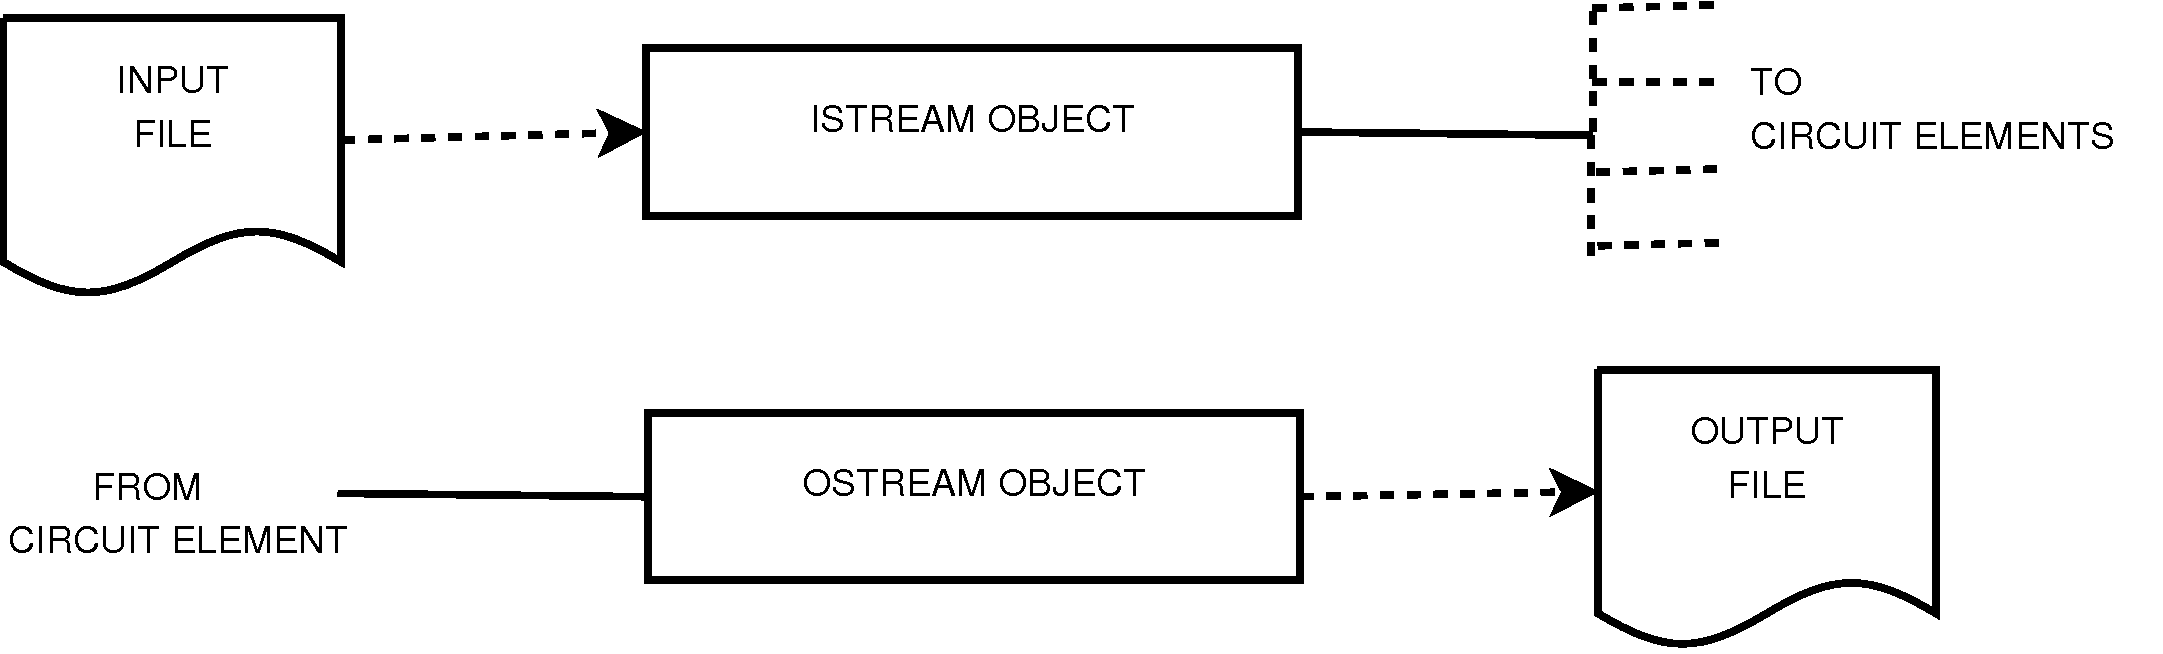
\includegraphics[scale=0.3]{iostream.png}
    \caption{{I/O Stream Model}}
  \label{iostream}
  \end{center}
  \end{figure}
 

\end{document}
